\chapter{\mypyvy}
\label{chap:mypyvy}

% Put this somewhere
%  % The project started because I wanted a clean sandbox in which
%  % to implement the \updr invariant inference algorithm~\cite{updr-jacm}.

\section{Introduction}

\begin{verbatim}
- something something invariant inference
- something something clean research platform
\end{verbatim}

\section{Background on Transition Systems}

\def\xMin{-8}
\def\xMax{8}
\def\yMin{-5}
\def\yMax{11}

\noindent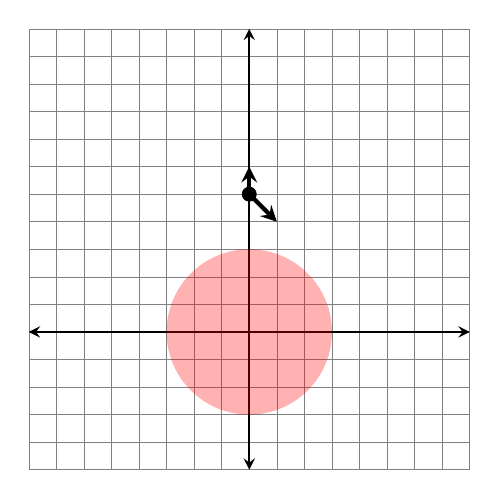
\begin{tikzpicture}[scale=0.35, >=stealth]
  \foreach \i in {\xMin,...,\xMax} {
      \draw [very thin,gray] (\i,\yMin) -- (\i,\yMax);
  }
  \foreach \i in {\yMin,...,\yMax} {
      \draw [very thin,gray] (\xMin,\i) -- (\xMax,\i);
  }
  \draw[<->, thick] (\xMin, 0) -- (\xMax, 0);
  \draw[<->, thick] (0, \yMin) -- (0, \yMax);
  \fill[fill=red, fill opacity=0.3] (0, 0) circle [radius=3];
  \draw[fill=black] (0, 5) circle [radius=0.25];
  \draw[->, line width=1.5pt] (0, 5) -- (0, 6);
  \draw[->, line width=1.5pt] (0, 5) -- (1, 4);
\end{tikzpicture} 
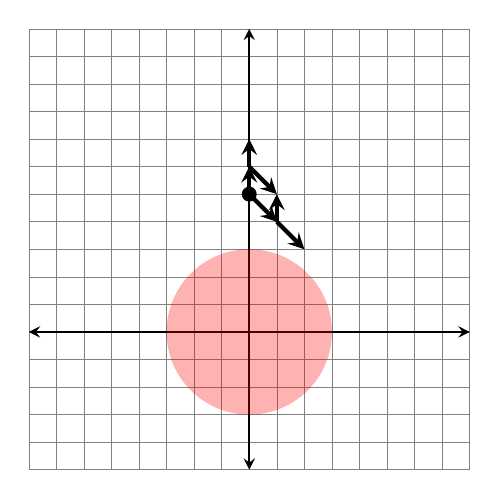
\begin{tikzpicture}[scale=0.35, >=stealth]
  \foreach \i in {\xMin,...,\xMax} {
      \draw [very thin,gray] (\i,\yMin) -- (\i,\yMax);
  }
  \foreach \i in {\yMin,...,\yMax} {
      \draw [very thin,gray] (\xMin,\i) -- (\xMax,\i);
  }
  \draw[<->, thick] (\xMin, 0) -- (\xMax, 0);
  \draw[<->, thick] (0, \yMin) -- (0, \yMax);
  \fill[fill=red, fill opacity=0.3] (0, 0) circle [radius=3];
  \draw[fill=black] (0, 5) circle [radius=0.25];
  \draw[->, line width=1.5pt] (0, 5) -- (0, 6);
  \draw[->, line width=1.5pt] (0, 5) -- (1, 4);
  \draw[->, line width=1.5pt] (0, 6) -- (0, 7);
  \draw[->, line width=1.5pt] (0, 6) -- (1, 5);
  \draw[->, line width=1.5pt] (1, 4) -- (1, 5);
  \draw[->, line width=1.5pt] (1, 4) -- (2, 3);
\end{tikzpicture} 
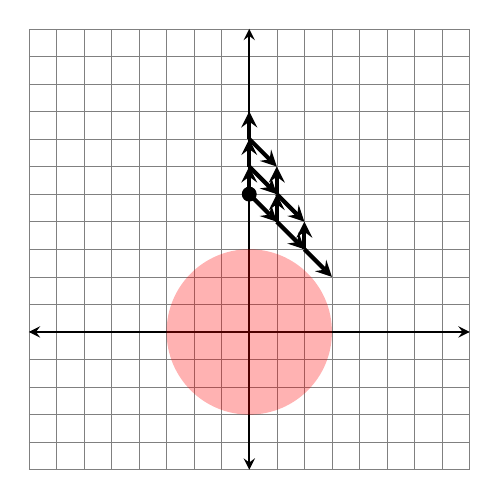
\begin{tikzpicture}[scale=0.35, >=stealth]
  \foreach \i in {\xMin,...,\xMax} {
      \draw [very thin,gray] (\i,\yMin) -- (\i,\yMax);
  }
  \foreach \i in {\yMin,...,\yMax} {
      \draw [very thin,gray] (\xMin,\i) -- (\xMax,\i);
  }
  \draw[<->, thick] (\xMin, 0) -- (\xMax, 0);
  \draw[<->, thick] (0, \yMin) -- (0, \yMax);
  \fill[fill=red, fill opacity=0.3] (0, 0) circle [radius=3];
  \draw[fill=black] (0, 5) circle [radius=0.25];
  \draw[->, line width=1.5pt] (0, 5) -- (0, 6);
  \draw[->, line width=1.5pt] (0, 5) -- (1, 4);
  \draw[->, line width=1.5pt] (0, 6) -- (0, 7);
  \draw[->, line width=1.5pt] (0, 6) -- (1, 5);
  \draw[->, line width=1.5pt] (1, 4) -- (1, 5);
  \draw[->, line width=1.5pt] (1, 4) -- (2, 3);
  \draw[->, line width=1.5pt] (0, 7) -- (0, 8);
  \draw[->, line width=1.5pt] (0, 7) -- (1, 6);
  \draw[->, line width=1.5pt] (1, 5) -- (1, 6);
  \draw[->, line width=1.5pt] (1, 5) -- (2, 4);
  \draw[->, line width=1.5pt] (2, 3) -- (2, 4);
  \draw[->, line width=1.5pt] (2, 3) -- (3, 2);
\end{tikzpicture}

\noindent\begin{tikzpicture}[scale=0.35, >=stealth]
  \foreach \i in {\xMin,...,\xMax} {
      \draw [very thin,gray] (\i,\yMin) -- (\i,\yMax);
  }
  \foreach \i in {\yMin,...,\yMax} {
      \draw [very thin,gray] (\xMin,\i) -- (\xMax,\i);
  }
  \draw[<->, thick] (\xMin, 0) -- (\xMax, 0);
  \draw[<->, thick] (0, \yMin) -- (0, \yMax);
  \fill[fill=red, fill opacity=0.3] (0, 0) circle [radius=3];
  \draw[fill=black] (0, 5) circle [radius=0.25];
  \fill[fill=green, fill opacity=0.3] (0, 5) -- (0, \yMax) -- (\xMax, \yMax) -- ($(\xMax,5)-(0,\xMax)$) -- cycle;
\end{tikzpicture} 
\begin{tikzpicture}[scale=0.35, >=stealth]
  \foreach \i in {\xMin,...,\xMax} {
      \draw [very thin,gray] (\i,\yMin) -- (\i,\yMax);
  }
  \foreach \i in {\yMin,...,\yMax} {
      \draw [very thin,gray] (\xMin,\i) -- (\xMax,\i);
  }
  \draw[<->, thick] (\xMin, 0) -- (\xMax, 0);
  \draw[<->, thick] (0, \yMin) -- (0, \yMax);
  \fill[fill=red, fill opacity=0.3] (0, 0) circle [radius=3];
  \draw[fill=black] (0, 5) circle [radius=0.25];
  \fill[fill=blue, fill opacity=0.3] (0, 5) -- ($(-\yMax,\yMax)+(5,0)$) -- (\xMax, \yMax) -- ($(\xMax,5)-(0,\xMax)$) -- cycle;
\end{tikzpicture} 
\begin{tikzpicture}[scale=0.35, >=stealth]
  \foreach \i in {\xMin,...,\xMax} {
      \draw [very thin,gray] (\i,\yMin) -- (\i,\yMax);
  }
  \foreach \i in {\yMin,...,\yMax} {
      \draw [very thin,gray] (\xMin,\i) -- (\xMax,\i);
  }
  \draw[<->, thick] (\xMin, 0) -- (\xMax, 0);
  \draw[<->, thick] (0, \yMin) -- (0, \yMax);
  \fill[fill=red, fill opacity=0.3] (0, 0) circle [radius=3];
  \draw[fill=black] (0, 5) circle [radius=0.25];
  \fill[fill=yellow, fill opacity=0.3] (0, 5) -- (0, \yMax) -- ($(-\yMax,\yMax)+(5,0)$) -- cycle;
\end{tikzpicture} 

\noindent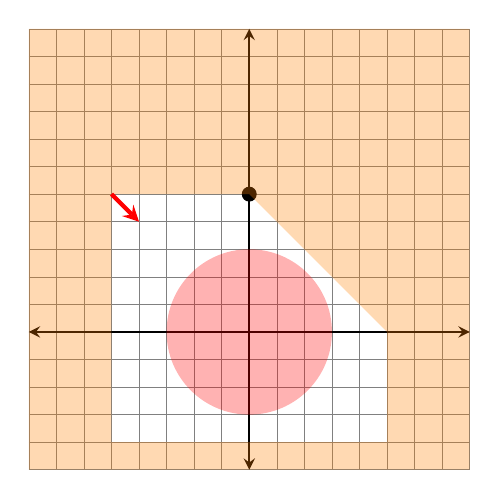
\begin{tikzpicture}[scale=0.35, >=stealth]
  \foreach \i in {\xMin,...,\xMax} {
      \draw [very thin,gray] (\i,\yMin) -- (\i,\yMax);
  }
  \foreach \i in {\yMin,...,\yMax} {
      \draw [very thin,gray] (\xMin,\i) -- (\xMax,\i);
  }
  \draw[<->, thick] (\xMin, 0) -- (\xMax, 0);
  \draw[<->, thick] (0, \yMin) -- (0, \yMax);
  \fill[fill=red, fill opacity=0.3] (0, 0) circle [radius=3];
  \draw[fill=black] (0, 5) circle [radius=0.25];
  \fill[even odd rule, fill=orange, fill opacity=0.3]
  (0, 5) -- (5, 0) -- (5, -4) -- (-5, -4) -- (-5, 5) -- cycle
  (\xMin, \yMax) -- (\xMax, \yMax) -- (\xMax, \yMin) -- (\xMin, \yMin) -- cycle;
  \draw[red, ->, line width=1.5pt] (-5, 5) -- (-4, 4);
\end{tikzpicture} 


\begin{verbatim}
- the crawler
  - thanks to jon howell for suggesting this example
  - cute little robot starting at (0, 5) in the plane
  - there is a circular hole of radius 3 centered at the origin
  - crawler can take 1 step due north or one diagonal step south-east
  - prove: the crawler never falls in the hole
  - model steps as binary relation on "states" (points in the plane)
  - a state s is reachable if there is some sequence of steps that starts from
    (0, 5) and ends at s
  - <draw nice pictures>
  - inductive invariant vs reachable states vs bad states
- mathematical transition systems
  - incrementally formalize the crawler in set theory
  - a transition system is a state space, a set of initial states,
    and a binary transition relation on states
  - an execution of a transition system is a nonempty sequence of states,
    the first of which is initial, and each adjacent pair of which are
    related by the transition relation.
  - a reachable state is one that appears in some execution
  - alternatively,
  - an invariant of a transition system is a set of states that contains
    all reachable states
  - the way to prove something is an invariant is by induction on executions.
  - an inductive invariant I is a set of states that:
    - contains all initial states
    - is closed under the transition relation;
      ie, if s \in I and s -> s' then s' \in I
  - the "safety verification problem for transition systems" is the problem of,
    given a transition system and a "goal" invariant called the safety property,
    find an inductive invariant that implies the safety property.
- first-order symbolic transition systems "on paper"
  - incrementally formalize the crawler in logic
  - so far everything is in math/set theory
  - can formalize transition systems in first-order logic as follows
  - states will be first-order structures over some vocabulary \sigma
  - initial states will be described by a FO-formula over \sigma
  - transition relation is a FO-formula over the "double vocabulary"
    consisting of two copies of \sigma, the second copy we call "primed"
  - the safety property is also a (single vocabulary) formula
  - the goal is to find a (single vocabulary) formula that is an inductive
    invariant for the system
  - inductiveness can be checked by checking validity of:
    - Init => I       (note: single vocab)
    - I /\ TR => I'   (note: double vocab)
      where I' is I with all the vocabulary symbols replaced by the primed copy
\end{verbatim}

\section{The Crawler in \mypyvy}

\begin{verbatim}
- incrementally formalize the crawler in \mypyvy
- make a joke about "mutable constant"
\end{verbatim}

\begin{verbatim}
mutable constant x: int
mutable constant y: int

init x = 0 & y = 5

transition north()
  modifies y
  new(y) = y + 1

transition south_east()
  modifies x, y
  & new(x) = x + 1
  & new(y) = y - 1

safety x * x + y * y > 9

invariant x + y >= 5
\end{verbatim}

\section{Expressing Transition Systems in \mypyvy}

\begin{verbatim}
- sort
- immutable/mutable relation/constant/function
- init
- transition
- modifies clauses
- all the expressions, k-stateness
- zero/one/twostate definitions
- attributes
- typechecking/inference
- implicit quantification of capitalized vars at outer scope
- note on implicit existential on transition params, but *not* defn params
- note on modifies clauses/frame conjuncts
\end{verbatim}

\section{Queries on Transition Systems}

\begin{verbatim}
- trace/bmc; the trace declaration; sat/unsat qualifier
- how to read states printed by mypyvy
- verify: invariant/safety
- zero/one/twostate theorem
- side note: custom printers using attributes
- updr
\end{verbatim}

\section{Internals of \mypyvy}

\begin{verbatim}
- a tour of main()
- the mental model of k-state formulas (correctly handling immutable)
  - evaluating a k-state formula on a trace
- philosophy on interacting with z3, the Solver class
- how to write a mypyvy "plugin"
- syntax.the_program and its consequences
\end{verbatim}

\section{Using \mypyvy}

\begin{verbatim}
- our port of the raft proof
- yotam's cav19
- jason's plid20
- pd
- derived relations?
- yotam's looking back algorithm or whatever it's called
\end{verbatim}

\section{Related Work}

\todo{introduce the expressiveness-automation spectrum, and place everybody on it}

\mypyvy is directly inspired by \ivy~\cite{Padon-al:PLDI16}.\footnote{
  \ivy's code is available on Github at \url{https://github.com/kenmcmil/ivy}.
  %
  See also the \ivy website at \url{http://microsoft.github.io/ivy/}.
}
%
The \ivy tool supports specification, implementation, and verification of systems,
including distributed and concurrent systems.
%
Systems are expressed as a set of \emph{actions},
each written in a simple imperative programming language
over state variables from a first-order vocabulary.
%
The verification queries \ivy asks of the underlying solver
are carefully designed to land in a decidable fragment of logic,
increasing the efficiency, reliability, and predictability
of the verification.
%
When verification fails, concrete counterexample traces
are shown to the user demonstrating the violation.
%
\ivy{} also has a powerful module system
that supports so-called ``circular'' assume-guarantee reasoning,
where all modules get to assume all other modules' invariants,
but are under the obligation to show that they do not violate
their own invariants.
%
(This reasoning is not actually circular, but sound,
because ``nobody violates their invariants first''
implies ``nobody violates their invariants''.)

One can view \mypyvy as similar to a hypothetical intermediate language
in \ivy{}'s pipeline to the solver.
%
\ivy{} compiles the modular imperative program
into a set of purely logical transition systems,
each of which must be verified.
%
One could imagine making this connection explicit,
by using \mypyvy as a ``backend'' for \ivy,
translating the transition systems into \mypyvy syntax.
%
This would have the advantage of making
\mypyvy's invariant inference algorithms available
to \ivy programs.
%
Indeed, many of the examples and benchmarks used by \mypyvy
were manually translated from \ivy.
%
We have begun work on such a translator,
and hope to continue to work more closely with \ivy in the future.


Dafny is a programming language
designed from the ground up for verification~\cite{Leino:LPAR10}.
%
Dafny is built on top of the Boogie intermediate verification language~\cite{boogie-manual},
which itself uses the Z3 SMT solver~\cite{z3}.
%
Dafny has an imperative object-oriented programming language with
objects, statements, loops, arrays, and heap-allocated data structures,
and has a rich Hoare logic for reasoning about these programs.
%
It also has a purely functional expression-oriented programming language
with first-class and higher-order functions, recursion, lists and logical quantifiers.
%
These logical features can be used express the specification of the imperative code,
or they can be used by themselves, turning Dafny into more of a proof assistant
than a programming language.
%
Dafny enjoys a high degree of proof automation, since all obligations are
eventually sent to Z3.
%
However, these queries can have complex quantifier structure to them, meaning
that they typically do not fall into any decidable fragment of first-order logic.
%
Dafny instructs Z3 to use syntactic heuristics based on E-matching
to manage quantifier instantiation process~\cite{z3-e-matching,simplify}.
%
This approach achieves good performance in practice,
but it means that the solver cannot return counterexamples,
and that the user must have a basic understanding of E-matching
in order to be an expert user of quantifiers in Dafny.

Previous chapters of this thesis used the \Coq proof assistant~\cite{Coq}.
%
\Coq is an interactive theorem prover and purely functional programming language
based on dependent type theory.
%
Its design gives it essentially limitless expressiveness,
but this comes at the cost of manual proof effort.
%
\Coq is the perfect tool for the job of building a new logic,
like we did in \cref{chap:disel} with \disel.
%
Also, \Coq has support for building domain-specific proof automation,
as promoted by \citet{chlipala:cpdt},
so with careful design, one can greatly reduce manual proof effort.
%
\mypyvy places itself at a very different point in the design space,
constraining what the programmer can write to a first-order transition system,
and in return, giving essentially full automation.
%
\todo{move the rest of this somewhere reasonable}
%
My own journey as a researcher has taken me through many points
on this spectrum.
%
I have seen the benefits of being able to transliterate
your mathematical theorem statements directly into a Coq proposition,
but I have also seen the beauty of not having to write any proofs.
%
In any particular domain, it often makes sense for the community to
begin by building tools in very expressive frameworks,
because we don't yet know what we will need.
%
After this initial step, researchers can start the process of
figuring out exactly what needs to be expressed,
and what can be traded away in exchange for better automation.

\TLA is a specification language for modeling systems
developed by \citet{lamport:tla,lamport:specifying-systems}.
%
It comes with a suite of tools to analyze models,
including tools for model checking and deductive theorem proving.
%
\citeauthor{lamport:tla} advocates for a style of using \TLA
where most of the benefit of the process is gained
just from formally expressing the model of the system,
because the user is forced to carefully think through the details.
%
Users can derive additional benefit by model checking their systems,
using the TLC bounded model checker~\cite{tlc}.
%
TLC is an explicit-state model checker that exhaustively explores
a finite version of the system (\eg, all Raft executions where
there at most 5 nodes, at most 2 commands, and at most 3 terms, etc.).
%
Users can go even further by using the \TLA proof system (TLAPS)
to prove their systems correct~\cite{tlaps}.
%
TLAPS uses a hierarchical (treelike) proof structure,
where the leaves of the tree can be dispatched by automated solvers.
%
The most interesting point of comparison for \mypyvy is
\TLA's language for specifying systems.
%
\TLA is much more expressive than \mypyvy,
allowing users to write arbitrary temporal logic formulas
to describe their system.
%
While sometimes needed, this expressiveness makes
analysis and proof more challenging,
and users often stay within an idiomatic subset that
constructs a transition relation as the finite disjunction of
parameterized actions.
%
One way to view \mypyvy is as a codification of this idiom into a language.
%
By restricting the way users write their system specifications,
\mypyvy is able to completely automatically analyze
the safety problem for these systems.
%
On the other hand, \mypyvy does not currently support liveness reasoning,
so users of \TLA would miss having access to that kind of reasoning.
%
We plan to investigate liveness in future work,
encoding the queries in first-order logic
following the approach of \citet{padon:reducing-liveness}.

nuSMV and nuXmv are symbolic model checkers,
originally based on BDDs and SAT solvers,
and later adopted to infinite-domain systems
by using SMT solvers~\todo{nusmv,nuxmv}.
%
These tools are ``workbenches'' that implement many different techniques
to attack the model checking problem.
%
This is similar in spirit to \mypyvy's goal of
providing a framework to implement several approaches.
%
One key difference between nuXmv and mypyvy is that
nuXmv's support for infinite-state systems
is based on integer and real number types,
while \mypyvy's primary way to reason about such systems
is based on pure first-order uninterpreted sorts.
%
In our experience, most distributed systems do not need
specific interpreted operations over numbers,
and instead are naturally expressed over uninterpreted sorts
using axioms for, e.g. a total order.

AVR is a recent word-level symbolic model checker
that has shown promise in the hardware model checking community~\cite{goel-avr}.
%
At its core, AVR uses syntax-guided abstraction to compute a
word-level model of the system in first-order logic,
which can then be analyzed with an implementation of IC3 on top of several SMT backend solvers
to infer an inductive invariant~\cite{bradley-ic3}.
%
Most closely related to \mypyvy is the subsequent tool I4~\cite{i4},
which builds on top of AVR's ability to efficiently verify finite-domain systems
to analyze infinite-state systems such as distributed protocols.
%
I4 works by constructing finite instances of the protocol,
analyzing them with AVR to get an inductive invariant for the finite protocol,
and then generalizing this invariant
to get a candidate invariant for the original protocol.
%
This candidate must then be verified using unbounded techniques,
such as \ivy~\cite{Padon-al:PLDI16},
and if a counterexample is obtained,
a larger finite instance of the protocol must be analyzed.
%
I4 reads protocols written in the \ivy input language.

Verification modulo theories (VMT)~\cite{nuxmv-user-manual,vmt-website}
is an extension of the SMT-LIB standard~\cite{smtlib-standard}
to support reasoning about symbolic transition systems.
%
Transition systems are defined by annotating a standard SMT-LIB function definition
with a special keyword marking it as the definition of the
initial conditions or transition relation.
%
Since transition relations are two-state formulas,
as discussed in~\todo{refer back to mypyvy discussion},
VMT again uses special keywords to declare that a SMT-LIB variable is
the ``next'' variable corresponding to another variable.
%
Both safety properties (of the form $\Box\varphi$) and
liveness properties (of the form $\Diamond\Box\varphi$)
can also be specified in the VMT description of the transition system,
but other queries (such as bounded reachability queries or
\mypyvy-style ``trace'' queries) cannot be specified.

\mypyvy's $k$-state semantics for formulas is
related to interpretations of Linear Temporal Logic (LTL)
over finite traces~\cite{vardi-ltl-finite}.
%
A key difference in the \mypyvy setting is that
each state is a first-order structure,
rather than a propositional truth assignment.
%
It would be interesting to extend \mypyvy
with explicit temporal operators that are ``unrolled''
when translating to the solver.

Btor2 is a language for specifying word-level hardware model checking problems
over bitvectors and arrays~\cite{btor2}.
%
It is an extension of the well-known bit-level format AIGER~\cite{aiger-1.9},
which is used in the hardware model checking competition~\cite{hwmcc20}.
%
Both AIGER and Btor2 are tailored to the case of reasoning
about finite-state systems, especially those derived from hardware designs.
%
Thus, neither supports infinite or unbounded sorts,
which is the focus of \mypyvy.

\section{Future Work}

\begin{verbatim}
- future directions in internals:
  - collapsing the many kinds of queries into one
  - handling transition declarations more uniformly (exists, modifies)
  - introducing a "logic" layer or other IR, or do less at z3 level
  - revisiting the "one program" mindset
\end{verbatim}

\section{Conclusion}

\begin{verbatim}
- call to arms for collaborators, builders-on-toppers, and users
- vision blah blah about verification UX and "exploration" of a TS,
  saving progress from run to run, "workbench"
\end{verbatim}